\section{Experimentación}

Presentaremos en esta sección la experimentación y discusión juntas, para cada experimento. Primero daremos una breve descripción de la instancia experimental, seguido de lo que esperamos observar, es decir, nuestra hipótesis. A continuación mostraremos los 
resultados obtenidos y nuestro análisis respecto a por qué obtuvimos dichos resultados.

\subsection{Metodología en la generación de instancias}

Para la creación de instancias de prueba, por una cuestión de practicidad, y para evitar sesgar los experimentos, decidimos utilizar instancias generadas aleatoriamente utilizando numpy. Todo el código de generación de datos, así como de corrida de tests, y las instancias utilizadas para la experimentación, se encuentran en la carpeta experimentos. En términos de las distribuciones utilizadas, en cada uno de los experimentos explicaremos las particularidades de la elección de distribución, pero aquí presentamos una tabla mostrando la distribución utilizada para la generación de los parámetros de las sanguijuelas:

\begin{center}
\begin{tabular}{l | l | l | l | l | l | l}
Experimento & Instancia & \#Sanguijuelas & X & Y & Radio & Temperatura\\ \hline
$1$ & $1$ & $50$ & $\mathcal{U}(45, 55)$ & $\mathcal{U}(45, 55)$ & $|\mathcal{N}(0.5, 10)|$ & $\mathcal{E}(1/100)$\\ \hline
$1$ & $2$ & $50$ & $\mathcal{U}(0, 100)$ & $\mathcal{U}(0, 100)$ & $|\mathcal{N}(2, 100)|$ & $\mathcal{E}(1/100)$\\ \hline
$1$ & $3$ & $50$ & $\mathcal{U}(0, 100)$ & $\mathcal{U}(0, 100)$ & $|\mathcal{N}(0.1, 10)|$ & $\mathcal{E}(1/300)$\\ \hline
$2$ & $1$ & $50$ & $\mathcal{U}(0, 100)$ & $\mathcal{U}(0, 100)$ & $\mathcal{U}(0, 10)$ & $\mathcal{E}(1/300)$\\ \hline
$3$ & $1$ & $31$ & Explicado & Explicado & Explicado & $\mathcal{E}(1/300)$\\ \hline
\end{tabular}
\end{center}

Todas las instancias son de $100x100$. En el caso del experimento 3 tomamos $h = 1$ para simplificar la generación de instancias, mientras que en los otros casos utilizamos

$$h \in \{0.5, 0.8, 1.0, 1.25, 2.0, 2.5, 4.0, 5.0, 6.25, 10.0, 12.5\}$$

Explicaremos más en profundidad estas decisiones en las subsecciones correspondientes. La elección de los valores de $h$ fue una tarea complicada: la restricción de $h | a \wedge h | b$ restringe ampliamente el conjunto de valores; fuera de eso, utilizar valores de granularidad demasiado pequeños aumenta demasiado el costo computacional, como veremos más adelante. Encontramos que intentar correr las instancias con un $h < 0.5$ elevaba demasiado el costo temporal de resolver el problema, por lo que utilizamos este valor como punto de comienzo.

\subsection{Experimento 1: temperatura en función de la granularidad}

Para este experimento, nos planteamos como objetivo estudiar la relación entre la matriz de temperaturas final, la granularidad, y la distribución de las sanguijuelas. Desde el punto de vista algorítmico, notemos que la granularidad impacta en las sanguijuelas que terminan determinando la temperatura inicial de los puntos: si una sanguijuela es lo suficientemente chica y está ubicada de forma tal que su radio no llega a impactar en el punto de la discretización más cercano, no será considerada como parte de la matriz. Más aun, es importante advertir que las elecciones impuestas sobre el modelado generan condiciones extrañas: cuando dos sanguijuelas se superponen en un punto, se tomará el máximo de las temperaturas como la inicial para el punto. Es decir, existen instancias donde el aumento de granularidad (y por lo tanto la aparición de sanguijuelas de radio pequeño) efectivamente termina borrando sanguijuelas que antes existían, reemplazándolas por otras de mayor temperatura. Lo que buscamos remarcar con esto es que es difícil predecir el efecto que va a tener el cambio de granularidad sobre la matriz final de temperaturas cuando comienzan a haber más sanguijuelas, ya que la interacción de la discretización con las mismas se vuelve cada vez más complicada.

El primer experimento que ideamos consiste en crear una instancia donde todas las sanguijuelas estén muy cercanas al punto crítico, con radios lo suficientemente pequeños como para que el efecto de desaparición que mencionamos antes logre entrar en acción. Tras un largo proceso de prueba y error, determinamos que las distribuciones mencionadas anteriormente eran las que mejor modelaban la idea intuitiva que estábamos buscando probar. En particular, la elección de una distribución exponencial se debe a que buscamos que las sanguijuelas tengan valores relativamente pequeños para que borrarlas logre mostrarnos un cambio concreto en la temperatura del punto crítico. Para todos los casos del experimento 1 utilizamos el método de eliminación gaussiana para obtener las matrices de temperatura correspondientes.

Intuitivamente esperábamos que la temperatura en el punto crítico fuera aumentando a medida que achicásemos el $h$: suponíamos que aumentar la granularidad forzosamente iba a resultar en que la mayor temperatura de las sanguijuelas cercanas al centro tomase relevancia en el punto crítico e iba a hacer que la temperatura del mismo subiese, mientras que tener una menor granularidad debía hacer que cada vez más sanguijuelas se perdieran en la discretización y forzaría a que las sanguijuelas mejor posicionadas para los nuevos valores de $h$ dominen la temperatura en el punto crítico. De las instancias que corrimos, creemos que el gráfico \ref{fig:exp11} es ampliamente representativo.

\begin{figure}[b]
    \centering
    \includegraphics[width=0.685\textwidth]{experimento 1-1}
    \caption{Variación de la temperatura en función de la granularidad para la primera instancia}
    \label{fig:exp11}
    
    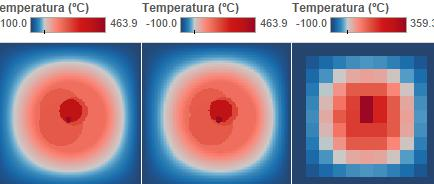
\includegraphics[width=0.685\textwidth]{Ejemplo Instancia 1}
    \caption{Mapa de calor para la instancia 1}
    \label{fig:exp11-vis}
\end{figure}

Es fácil observar que la temperatura del punto critico se estabiliza a medida que aumenta la granularidad, y tiende a ser más bien caótico a medida que aumentamos el valor de h, es decir, disminuimos la granularidad. A diferencia de lo que esperábamos, la temperatura con mayor granularidad no es la mayor de las obtenidas, encontramos que la granularidad de la discretización es más bien un parámetro de regulación para la precisión de la solución: cuanta mayor granularidad, más difícil es que las sanguijuelas que aparezcan cambien sustancialmente la temperatura del punto crítico, ya que un $h$ más pequeño implica que los radios de las sanguijuelas que quedan por descubrir son lo suficientemente chicos como para afectar pocos puntos, y la ecuación de calor parece "balancear" las temperaturas hacia los valores más frecuentes. A modo de ayudar a la comprensión del experimento y la instancia contemplada, creamos una visualización del mapa de temperaturas generado por esta instancia particular, variando los valores de $h$:

Observemos que a medida que disminuimos la granularidad, el borde con temperatura $-100$ºC comienza a tomar cada vez más relevancia dentro de la discretización, y colabora aun más que antes a reducir los valores de temperatura.

\pagebreak

Para la segunda instancia pensamos en crear sanguijuelas de un radio grande, en comparación con la primera instancia, alejadas del punto critico. En este caso esperábamos, en principio, que la temperatura se mantuviese constante a medida que aumentamos la granularidad, pues las sanguijuelas son lo suficientemente grandes para no desaparecer dentro de la discretización y más aun, esperamos una variación pequeña de temperatura en relación al aumento del $h$. Observemos que en este caso cambiamos completamente la forma de generar las instancias de test, quitando restricciones en tanto a los valores de las sanguijuelas: el hecho de tomar distribución uniforme para las posiciones nos asegura la existencia de sanguijuelas en una variedad de puntos de la discretización, mientras que el radio normal nos da acceso a un panorama más variado en términos de los radios.

\begin{figure}[b]
    \centering
    \includegraphics[width=0.685\textwidth]{experimento 1-2}
    \caption{Variación de la temperatura en función de la granularidad para la segunda instancia}
    \label{fig:exp12}
    
    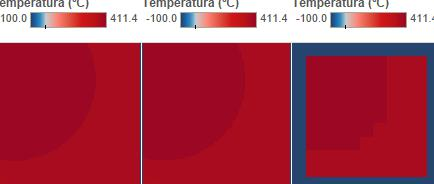
\includegraphics[width=0.685\textwidth]{Ejemplo Instancia 2}
    \caption{Mapa de calor para la instancia 2}
    \label{fig:exp12-vis}
\end{figure}

La justificación de porque la temperatura se estabiliza cercano a los $410$ºC es por qué hay una sanguijuela de aproximadamente $411$ºC y un radio muy grande, eso hace que abarque a muchos puntos de la discretización por más variación del h que haya. Con su radio, llega hasta el punto crítico y siempre le gana en temperatura a las sanguijuelas cercanas, ya que es la de mayor temperatura en esta instancia, y eso hace que le aumente la temperatura a los puntos de la discretización que no tienen sanguijuelas cercanas, como por ejemplo los puntos cercanos al centro del parabrisas pero que están del otro lado de la sanguijuela más caliente y no tienen ninguna sanguijuela a su alrededor. Al promediarse la temperatura en esos puntos, hace que la temperatura en el punto crítico sea cercana a los $410$ºC.

Observemos, en la figura \ref{fig:exp12}, que efectivamente la diferencia de temperatura entre el primer y el último h es baja, menor a $5$ºC, confirmando nuestra hipótesis sobre la variación de la temperatura a lo largo del aumento de granularidad. Una vez más encontramos que el algoritmo converge a una solución a partir de cierto $h$ y se mantiene estable, aunque la diferencia en este caso es que el $h$ viene antes que en la instancia 1. Una vez más, proveemos una visualización de la clase generada para la instancia 2 en el gráfico \ref{fig:exp12-vis}

\pagebreak

Como tercera instancia, nos planteamos ver qué sucede con las sanguijuelas más pequeñas al estar alejadas del centro. Para esto, generamos instancias con las distribuciones mencionadas anteriormente, pero observemos que en este caso tomamos la temperatura como una variable exponencial de esperanza $300$, es decir, tomamos valores de temperatura mucho más altos. Nuestro análisis de los casos anteriores nos induce a pensar que las sanguijuelas suficientemente peque\~nas no tendrán tanta relevancia en la temperatura del punto critico. Esto es porque, al afectar pocos puntos de la discretizaci\'on, la ecuación de calor compensa esos valores al alejarse de la posición de las sanguijuelas. 

\begin{figure}[b]
    \centering
    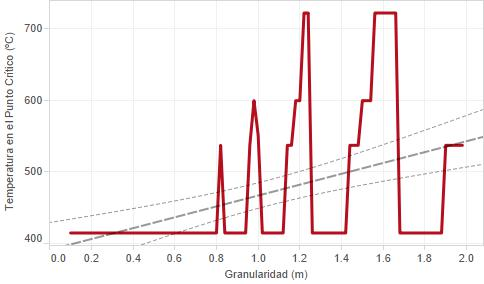
\includegraphics[width=0.685\textwidth]{experimento 1-3}
    \caption{Variación de la temperatura en función de la granularidad para la tercera instancia}
    \label{fig:exp13}
    
    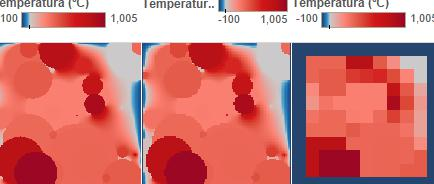
\includegraphics[width=0.685\textwidth]{Ejemplo Instancia 3}
    \caption{Mapa de calor para la instancia 3}
    \label{fig:exp13-vis}
\end{figure}

En el gráfico \ref{fig:exp13} podemos observar que la temperatura solo varia, para una granularidad muy baja, en el orden de los $20$ºC. Sin embargo, a diferencia de los casos anteriores, encontramos que la temperatura se estabiliza a valores cada vez mas bajos al aumentar la granularidad, que efectivamente es lo que hipotetizamos que sucedería. Para profundizar la comprensión, podemos ver en el gráfico \ref{fig:exp13-vis} los mapas de calor correspondientes a la tercera instancia.
\\
   Al tener un radio tan chico la mayoría de las sanguijuelas, por más alta que sea su temperatura, no va a afectar a gran cantidad de puntos. Por ejemplo tenemos la sanguijuela de temperatura máxima que es de $1000$ºC, sin embargo,  por más distinta que sea la discretización, la temperatura nunca supera los $270$ºC (para los valores de h probados), ya que al estar tan separada del centro y no tener un radio tan grande, no abarca muchos puntos de la discretización y la temperatura se va perdiendo a medida que nos vamos acercando al punto crítico.
\\
Nótese a medida que aumenta la granularidad la disipación de temperatura aumenta. En particular, nos concentramos en las sanguijuelas de mayor temperatura. Vemos que, en el mapa de mayor granularidad, parece que los altos valores de temperatura se limitan al área cubierta por las mismas, mientras que la temperatura desciende drásticamente al salir del radio. Se puede, sin embargo, observar áreas de calor entre dos sanguijuelas relativamente cercanas, donde la función de disipación debe disipar calor en dos direcciones contrarias. Observado esto, solo podemos concluir que las sanguijuelas de mayor temperatura están demasiado alejadas entre si, por lo que las altas temperaturas se pierden automáticamente en la ecuación.

Naturalmente, el algoritmo de factorización LU debería devolver exactamente las mismas matrices de temperatura (ya que resuelven el mismo problema). Comprobamos de cualquier forma en nuestra experimentación que esto funcionaba así como forma de testear la correctitud del código fuera de las instancias provistas por la cátedra.

\pagebreak

\subsection{Experimento 2: relación entre tiempo de cómputo y calidad de la solución}

Para este experimento, buscábamos complementar los conocimientos adquiridos en el experimento anterior: sabíamos que cuanta mayor granularidad teníamos, más precisa es nuestra solución, y teníamos claro que tomar valores de $h$ muy pequeños no nos permitía solucionar los problemas por la excesiva carga computacional. Ahora lo que faltaba entender mejor es cuál es la relación entre el costo computacional y la granularidad. Para esto, utilizamos la tercera instancia que habíamos creado en el experimento anterior y medimos los tiempos de ejecución del algoritmo, la metodología utilizada fue correr el programa $5$ veces por cada valor de $h$, y tomar el promedio de los tiempos reportados.

En el gráfico \ref{fig:exp21} podemos observar, en el primer casillero, la comparación entre los algoritmos, mientras que el segundo muestra la dimensión de la matriz del sistema a resolver (un punto $(h, d)$ en el gráfico se corresponde con una matriz final de $d \times ([\frac{a}{h}] + 1)$, tomaremos de aquí en adelante a $n$ como este $d$). Observemos que las filas de la matriz del sistema crecen a la razón de $f(h) = ([\frac{a}{h}] + 1)([\frac{b}{h}] + 1)$, que es una función decreciente, con límite a $+\infty$ cuando $h$ tiende a $0$. Es importante destacar que este gran crecimiento de la matriz impacta muy fuertemente sobre el costo computacional, ya que ambos algoritmos son $O(n^3)$ a pesar de las mejoras que alcanzamos explotando la estructura de banda de la matriz.

En concreto, tenemos que el costo de realizar eliminación gaussiana y resolver el sistema usando backward substitution es de $\frac{2n^3}{3} + \frac{3n^2}{2} + O(n)$ para sistemas que no precisan hacer pivoteo ~\cite{burden} (cabe destacar que esto no contempla las optimizaciones que realizamos para explotar la estructura de banda). Mientras tanto, realizar la factorización LU y resolver utilizando forward y backward substitution toma $\frac{2n^3}{3} + 2n^2 + O(n)$ ~\cite{LUComplexity}. Observemos que el costo de la factorización LU es mayor por un sumando de $\frac{n^2}{2}$, pero la explosión de complejidad que terminamos teniendo en las filas de la matriz hacen que este $n$ se dispare, generando la amplia diferencia que vemos en el gráfico \ref{fig:exp21}.

\begin{figure}[b]
    \centering
    \includegraphics[width=0.685\textwidth]{experimento 2-1}
    \caption{Comparación entre EG y LU}
    \label{fig:exp21}
\end{figure}



\pagebreak

\subsection{Experimento 3: comparación entre algoritmos para eliminación de sanguijuelas}

En este experimento nos enfocamos en analizar las diferencias entre los algoritmos de eliminación de sanguijuelas, a los que llamaremos eliminación simple y eliminación con Sherman-Morrison. Basados en los tests de correctitud, podemos afirmar que ambos algoritmos tienen el mismo comportamiento cualitativo. Es decir, ambos devuelven la misma solución. Por esto, el enfoque de este experimento es el análisis temporal de los experimentos. 

Antes de establecer hipótesis alguna, vamos a hacer un breve análisis del comportamiento esperado de cada algoritmo.

En primer lugar tenemos el algoritmo de eliminación simple. Este algoritmo se limita a, iterando sobre todas las sanguijuelas, eliminar una y recalcular la matriz de temperatura. Este comportamiento es independiente de los atributos de las sanguijuelas en si, sino que, a primera vista, es esperable que la complejidad solo dependa de la cantidad de sanguijuelas.

Luego tenemos eliminación con Sherman-Morrison. En este caso, si se vuelve relevante el radio de las sanguijuelas, ya que este algoritmo se evita recalcular toda la factorizaci\'on si la sanguijuela afecta solo un punto de la discretizaci\'on. 

Es por esto, que dise\~namos nuestro experimento de modo que se pueda apreciar la diferencia en el modo de cómputo. Este consiste en un tablero de $100 \times 100$ mts$^2$, en el cual fijaremos la cantidad de sanguijuelas y el tamaño de la discretizaci\'on. Para medir la performance de cada algoritmo, vamos a variar el radio de las sanguijuelas. Es decir, variaremos el porcentaje de sanguijuelas que solo afectan a un punto de la discretizaci\'on. Generamos instancias con $31$ sanguijuelas, incrementando el porcentaje de sanguijuelas unitarias que se encontraban en cada instancia con diferencias de aproximadamente $10\%$. Todas las instancias se caracterizan por tomar $h = 1$, y disponer de las sanguijuelas en forma de grilla, es decir, ocupando las posiciones en orden desde la esquina inferior derecha por filas, hasta lograr cubrir las posiciones necesarias. Además, posicionamos una sanguijuela de $1000$ºC en el punto crítico, para asegurarnos que los algoritmos corran al tener la misma por encima de $235$ºC. La forma de generar sanguijuelas unitarias es, entonces, a través de tomar radios menores a $0.8$ y mayores a $0.2$, mientras que en el caso dual podemos tomar sanguijuelas de radio mayor a $1.1$ y menor a $1.4$. Observemos que el incremento podemos determinarlo como "aproximadamente" de $10\%$ debido a que las sanguijuelas "unitarias" que se encuentren en el límite con las sanguijuelas no unitarias van a tener su posición influenciada por más de 1 sanguijuela, haciendo que no pueda aplicarse Sherman Morrison. De cualquier forma, esta limitación no generó ninguna complicación, ya que el cambio en el porcentaje es lo suficientemente bajo como para poder analizar los resultados de la misma forma. 

\begin{figure}[h]
    \centering
    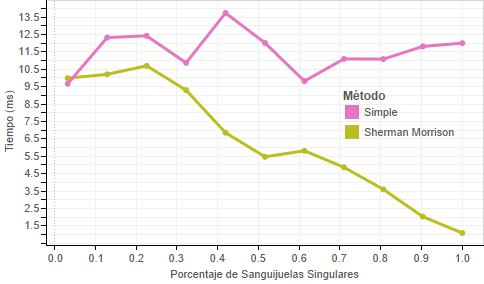
\includegraphics[width=0.685\textwidth]{experimento 3-1}
    \caption{Comparación entre SM y el método simple}
    \label{fig:exp31}
\end{figure}

Si miramos los tiempos de ejecución para Sherman-Morrison, podemos observar claramente que a medida que aunmenta el porcentaje de sanguijuelas unitarias, el tiempo de computo disminuye. Esto se debe a que cada vez que debe analizar una sanguijuela unitaria, puede aprovechar los resultados ya calculados, en lugar de recalcular la matriz entera, derivando en un menor costo computacional a medida que disminuye el radio de las sanguijuelas.

Por su parte, el algoritmo de elimacion simple mantiene un rango bajo de variacion en las mediciones. Esto sucede porque independientemente del rango de las sanguijuelas, siempre debe recalcular el total de los datos al eliminar una. 

Si comparamos la primer medicion, donde todas las sanguijuelas afectan mas de un punto de la discretizacion, podemos notar que eliminacion con Sherman-Morrison

